%-----------------------------
\chapter{\label{key:latexsample}Diferentes exemplos num único capítulo}

Esta é a segunda versão do documento utilizado como template para o relatório de trabalhos e/ou projetos desenvolvidos para cada uma das Unidades Curriculares da Licenciatura de Engenharia de Sistemas Informáticos na Escola Superior de Tecnologia\footnote{\url{https://est.ipca.pt/}}.


\noindent\fbox{%
	\parbox{\textwidth}{%
		\textcolor{red}{NOTA: Documento em construção! Este capítulo~\ref{key:latexsample} deve ser removido na versão final deste documento...}
	}%
}


%-----------------------------
\section{Preparar o ambiente LaTeX}

Assumindo que estás a utilizar o sistema operativo Windows, para editares documentos \LaTeX\ necessitas de instalar as seguintes ferramentas:
\begin{itemize}
	\item \textbf{MiKTeX}\footnote{\url{https://miktex.org/}}, esta ferramenta funciona na linha de comandos (de um terminal) e disponibiliza um conjunto de comandos necessários para compilar o código e produzir o documento final. No repositório tens dois scripts\footnote{no formato \textit{batch processing file}, mas também foram criados para utilizar num terminal do MacOS} para gestão do projeto:
	\begin{itemize}
		\item \textbf{tex-win-make.bat} executa a sequência completa para compilar o projeto;
		\item \textbf{tex-win-clear-temp-files.bat} limpa os ficheiros desnecessários criados durante a compilação do projeto.
	\end{itemize}
	\item \textbf{TeXstudio}\footnote{\url{https://texstudio.org/}}, é um excelente IDE para \LaTeX.
\end{itemize}


%-----------------------------
\section{Utilizar referências}

Este capítulo fala de \gls{stemmer}s. Mas não esquecer os \Gls{lematizador}es

O \acrfull{http} é um protocolo baseado em \acrshort{tcp}.

Citar o livro "The Art of Computer Programming"\cite{knuth1973}.

A introdução está colocada na página \pageref{key:introducao}.


%-----------------------------
\section{Secção}

Blá, blá, blá...

\colorbox{Red}{documento em construção...}

\subsection{Subsecção}

Blá, blá, blá...

\textbf{\textcolor{Red}{documento em construção...}}


\subsubsection{Subsubsecção}

Blá, blá, blá...


%-----------------------------
\section{Utilizar lista1}
Texto de suporte para um exemplo de utilização de lista.

\begin{itemize}
	\item Item 1;
	\item Item 2; 
	\item Item 3;
	\item Conclusão.
\end{itemize}{}


%-----------------------------
\section{Utilizar lista2}
Texto de suporte para outro exemplo de utilização de lista.

\begin{enumerate}
	\item Item 1;
	\item Item 2; 
	\item Item 3;
	\item Conclusão.
\end{enumerate}{}

%-----------------------------
\section{Exemplo de colocação de figuras}

Ao contrário do Word, o \LaTeX{} usa um mecanismo de colocação de figuras e tabelas em que estas flutuam ao longo das páginas de acordo com a necessidade/disponibilidade em termo de espaço vertical.
Assim, não devem usar frases como ``na figura acima'', ou ``na figura abaixo'', mas fazer referências:
``tal como se pode observar na Figura~\ref{fig:1}'' (a figura poderá estar numa página diferente, portanto se for muito importante indicar a página, necessitas apenas de colocar a referência para essa página \pageref{fig:1} caso seja pertinente e necessário).

\begin{figure}[htb]
	\centering
	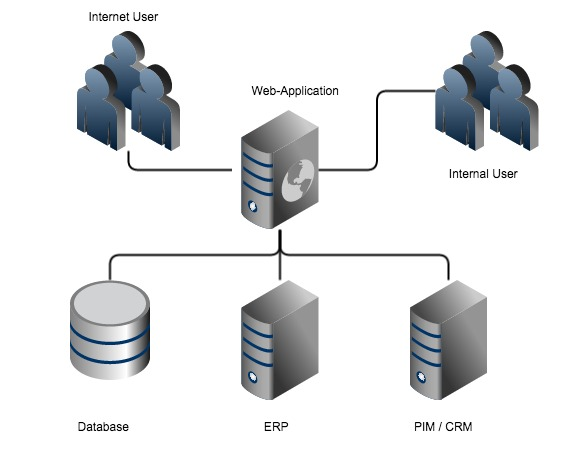
\includegraphics[width=0.8\linewidth]{img/sample}  % largura percentual 
	\caption{Figura para o exemplo}
	\label{fig:1}
\end{figure}


%-----------------------------
\section{Exemplo de tabela}
Texto de suporte para um exemplo de tabela.

O mesmo acontece com as tabelas, como se pode ver na Tabela~\ref{tab:1} (a tabela poderá estar numa página diferente, portanto se for muito importante indicar a página, necessitas apenas de colocar a referência para essa página \pageref{tab:1} caso seja pertinente e necessário).

\begin{table}[htb]
	\centering
	\begin{tabular}{ccccc}
		\toprule
		\textbf{A} & \textbf{B} & \textbf{C} & \textbf{D} & \textbf{Total} \\
		\midrule
		1 & 2 & 3 & 4 & 10  \\
		2 & 3 & 4 & 5 & 14  \\
		3 & 4 & 5 & 6 & 18  \\
		4 & 5 & 6 & 7 & 22  \\
		\bottomrule
	\end{tabular}
	\caption{Tabela exemplo}
	\label{tab:1}
\end{table}


%-----------------------------
\section{Utilizar Verbatim}
Texto de suporte para o exemplo de utilização do bloco Verbatim.

\subsection{Lista dos carateres a ignorar}
\begin{Verbatim}
  t_ignore = " \t\n"
\end{Verbatim}
\hfill \break

%-----------------------------
\section{Utilizar listagem de programa}
Texto de suporte para o exemplo de utilização de listagem.

\subsection{Listagem de programa em C\#}
Para a inclusão de código, usa-se algo semelhante. Veja-se a Listagem~\ref{lst:1}.

\begin{lstlisting}[language={[sharp]c},
caption={Método para contar o número de elementos numa lista iguais a uma determinada string.},
label=lst:1]
  public int count(string x) {
    return items.Select( y => y == x ).Count();
  }
\end{lstlisting}

\subsection{Listagem de programa em C}
Outro exemplo de código, usa-se algo semelhante. Veja-se a Listagem~\ref{lst:p1e}.

\begin{lstlisting}[language={c},
	caption={Código do programa: \textbf{apaga}.},
label=lst:p1e]
/**
* programa apaga.c
* @author #20808 Joao Carlos Pinto
*/
#include <stdio.h>
#include <unistd.h>
#include <errno.h>
#include <string.h>
#include "mytools.h"

int main(int argc, char *argv[]) {
  char buffer[MAXBUFFERSIZE];
  if (argc < 2) {
    buffer[0] = '\0';
    sprintf(buffer, "Falta: ficheiro\n Deve "+
    "utilizar-se desta forma:\n%s ficheiro(s)\n", 
    argv[0]);
    escrevErro(buffer);
    return 1;
  }
  int resultado, bkErrno;
  for(int i=1; i<argc; i++){
    if ((resultado = unlink(argv[i])) == -1) {
      buffer[0] = '\0';
      bkErrno = errno;
      sprintf(buffer, "erro (%d, %s) ao apagar o "+
      "ficheiro: %s\n", bkErrno, strerror(bkErrno), 
      argv[i]);
      escrevErro(buffer);
      return 1;
    }
    if (resultado == 0) {
      buffer[0] = '\0';
      sprintf(buffer, "o ficheiro \"%s\" foi apagado!\n", 
      argv[i]);
      escrever(buffer);
    } else {
      buffer[0] = '\0';
      bkErrno = errno;
      sprintf(buffer, "resultado (%d, %s) inesperado ao "+
      "apagar o ficheiro \"%s\"!\n", bkErrno, 
      strerror(bkErrno), argv[i]);
      escrevErro(buffer);
      return 1;
    }
  }
  return 0;
}
\end{lstlisting}

